\documentclass{beamer}
%\documentclass[handout]{beamer}

\usepackage[utf8x]{inputenc}
\usepackage{color}
\usepackage{multirow}
\usepackage{graphicx}

\usetheme{Boadilla}
\usefonttheme{professionalfonts}
\useoutertheme[subsection=false,footline=empty]{miniframes}
\useinnertheme{circles}
\setbeamertemplate{footline}[frame number]

\author{Roland Hieber}
\title{Das Network~Time~Protocol und Stratum~0}
\institute{Stratum~0~e.~V.}
\date{31.~Januar~2012}

\begin{document}
\begin{frame}
  \titlepage
  \thispagestyle{empty}
\end{frame}

\section{Motivation}
\begin{frame}{Motivation}
  \begin{itemize}
    \item Systemzeit kann von echter Zeit abweichen
    \item Uhren gehen unterschiedlich schnell
  \end{itemize}

  \pause

  \begin{block}{Lösung}
    \begin{itemize}
      \item Zeit von einem anderen System synchronisieren
      \item Systemuhr verlangsamen/beschleunigen
      \item[$\Rightarrow$] \texttt{ntpd} unter Unix tut genau dies
    \end{itemize}
  \end{block}
\end{frame}

\section{Protokoll}
\begin{frame}{Architektur}
  \begin{center}
    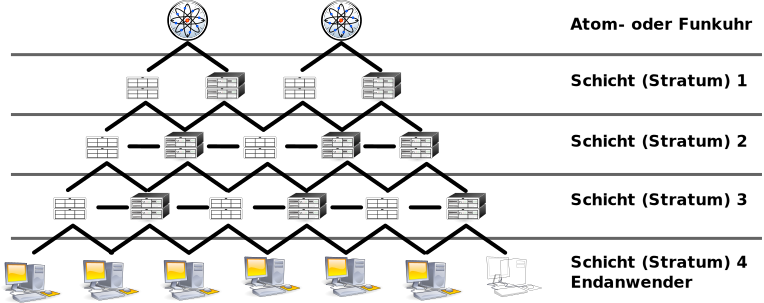
\includegraphics[width=\textwidth]{Architecture_NTP_labels_de.pdf}\par
    \tiny Bild: Public Domain,
    \url{http://de.wikipedia.org/wiki/Datei:Architecture_NTP_labels_de.svg}
  \end{center}
\end{frame}

\begin{frame}{Architektur}
  \begin{center}
    \includegraphics[width=\textwidth]{Architecture_NTP_Stratum0.pdf}\par
    \tiny Bild: Public Domain,
    \url{http://de.wikipedia.org/wiki/Datei:Architecture_NTP_labels_de.svg}
  \end{center}
\end{frame}

\begin{frame}{Atomuhr CS2 der PTB Braunschweig}
  \begin{center}
    \includegraphics[width=0.8\textwidth]{Atomuhr-CS2.jpg}
    \par\tiny Bild: Jörg Behrens, CC-BY-SA 3.0,
    \url{http://commons.wikimedia.org/wiki/File:Atomuhr-CS2.jpg}
  \end{center}
\end{frame}

\begin{frame}{Paketformat (NTPv4)}
  \begin{itemize}
    \item Transport über UDP, Port 123
  \end{itemize}
  \pause
  \footnotesize
  \ttfamily
  \begin{center}

    \begin{tabular}[h]{|*{32}{@{\,}c@{\,}}|}
      0 & 1 & 2 & 3 & 4 & 5 & 6 & 7 & 8 & 9 & A & B & C & D & E & F &
      0 & 1 & 2 & 3 & 4 & 5 & 6 & 7 & 8 & 9 & A & B & C & D & E & F\\
      \hline

      \multicolumn{2}{|@{\,}c@{\,}|}{LI} &
      \multicolumn{3}{|@{\,}c@{\,}|}{Ver} &
      \multicolumn{3}{|@{\,}c@{\,}|}{Mode} &
      \multicolumn{8}{|@{\,}c@{\,}|}{Stratum} &
      \multicolumn{8}{|@{\,}c@{\,}|}{Poll} &
      \multicolumn{8}{|@{\,}c@{\,}|}{Precision} \\
      \hline

      \multicolumn{32}{|@{\,}c@{\,}|}{Root Delay} \\ \hline
      \multicolumn{32}{|@{\,}c@{\,}|}{Root Dispersion} \\ \hline
      \multicolumn{32}{|@{\,}c@{\,}|}{Reference Clock ID} \\ \hline

      \multicolumn{32}{|@{\,}c@{\,}|}{
        \multirow{2}{*}{Reference Timestamp (64)}} \\
        \multicolumn{32}{|c|}{} \\ \hline
      \multicolumn{32}{|@{\,}c@{\,}|}{
        \multirow{2}{*}{\color{red} Origin Timestamp (64)}} \\
        \multicolumn{32}{|c|}{} \\ \hline
      \multicolumn{32}{|@{\,}c@{\,}|}{
        \multirow{2}{*}{\color{red} Receive Timestamp (64)}} \\
        \multicolumn{32}{|c|}{} \\ \hline
      \multicolumn{32}{|@{\,}c@{\,}|}{
        \multirow{2}{*}{\color{red} Transmit Timestamp (64)}} \\
        \multicolumn{32}{|c|}{} \\ \hline

      \multicolumn{32}{|@{\,}c@{\,}|}{Extension Fields} \\
      \multicolumn{32}{|@{\,}c@{\,}|}{\vdots} \\
    \end{tabular}
  \end{center}
\end{frame}

\begin{frame}{Zeitsynchronisation}
  \begin{center}
    \includegraphics[width=0.7\textwidth]{algo.pdf}
  \end{center}

  \pause

  \begin{itemize}
    \item[] Zeitdifferenz:
      $\theta = T(B) - T(A) = \frac12 * \left((t_2-t_1) + (t_3-t_4)\right)$
  \end{itemize}

\end{frame}

\section{Quellen}
\begin{frame}
  \centering
  \vfill
  Vielen Dank für die Aufmerksamkeit!
  \vfill
  {\footnotesize Diese Vortragsfolien sind lizenziert unter CC-BY-SA 3.0.}
  \vfill
  \begin{thebibliography}{9}
    \bibitem{rfc}{D. Mills et~al.: RFC 5905: \emph{Network Time Protocol
      Version 4: Protocol and Algorithms Specification},
      \url{https://tools.ietf.org/html/rfc5905}}
    \bibitem{wikipedia}{Wikipedia: \emph{Network Time Protocol},
      \url{http://en.wikipedia.org/w/index.php?oldid=469612852}}
  \end{thebibliography}

\end{frame}

\end{document}
